

%-------------------------------------------------------
%-------------------------------------------------------

\begin{frame}{1D Wave Propagation Algorithm (LeVeque et al.)}
	\scriptsize
	
	We consider the hyperbolic system
	\[
	q_t + f(q)_x = 0, \quad q \in \mathbb{R}^m
	\]
	
	\begin{itemize}
		\item Discretize the domain into cells $[x_{i-1/2}, x_{i+1/2}]$.
		\item At each interface $x_{i+1/2}$, solve the Riemann problem:
		\[
		q(x,0) = 
		\begin{cases} 
			q_i, & x < x_{i+1/2}, \\ 
			q_{i+1}, & x > x_{i+1/2}.
		\end{cases}
		\]
		\item Decompose the jump into waves along eigenvectors of $A = f'(q)$:
		\[
		q_{i+1} - q_i = \sum_{p=1}^m \alpha^p r^p, 
		\quad W^p = \alpha^p r^p, \; \text{travelling with } s^p.
		\]
		\pause
		\item Define fluctuations:
		\[
		\mathcal{A}^+ \Delta q_{i-1/2} = \sum_{p: s^p>0} s^p W^p, \quad
		\mathcal{A}^- \Delta q_{i+1/2} = \sum_{p: s^p<0} s^p W^p
		\]
		\item Update cell averages:
		\[
		Q_i^{n+1} = Q_i^n - \frac{\Delta t}{\Delta x} 
		\Big( \mathcal{A}^+ \Delta q_{i-1/2} + \mathcal{A}^- \Delta q_{i+1/2} \Big)
		\]
	\end{itemize}
\end{frame}



%-------------------------------------------------------
%-------------------------------------------------------

\begin{frame}{Multidimensional Wave Propagation (2D and 3D)}
	\scriptsize
	\begin{columns}[c]
		
		%------------------ Linke Spalte: Theorie ------------------%
		\begin{column}{0.55\textwidth}
			\textbf{General system:}
			\[
			q_t + f(q)_x + g(q)_y + h(q)_z = 0
			\]
			
			\textbf{Key ideas:}
			\begin{itemize}
				\item \textbf{1D Riemann problems at cell interfaces:}  
				Solve along the normal direction of each cell interface.
				\item \textbf{Wave decomposition:}  
				Decompose jumps into waves \(W^p\) with speeds \(s^p\).
				\item \textbf{Fluctuations:}  
				\[
				\mathcal{A}^\pm \Delta q, \quad 
				\mathcal{B}^\pm \Delta q, \quad 
				\mathcal{C}^\pm \Delta q
				\]
				\pause
				\item \textbf{Transverse propagation:}  
				\begin{itemize}
					\item 2D: Waves in \(x\)-direction generate waves in \(y\), and vice versa.
					\item 3D: Each wave generates transverse waves along in the other two directions.
				\end{itemize}
			\end{itemize}
		\end{column}
		
		%------------------ Rechte Spalte: 2D-Gitter ------------------%
		\begin{column}{0.45\textwidth}
			\centering
		  \begin{tikzpicture}[scale=1, every node/.style={font=\small}]
			% grid
			\def\n{3}
			\foreach \i in {0,...,\n} {
				\draw[thin] (\i,0) -- (\i,\n);
				\draw[thin] (0,\i) -- (\n,\i);
			}
			
			% highlight cell (i,j)
			\fill[blue!12] (1,1) rectangle (2,2);
			\coordinate (C) at (1.5,1.5);
			\node at (1.5,1.5) {$(i,j)$};
			
			% interfaces (thick)
			\draw[thin] (1,1) -- (1,2);
			\draw[thin] (2,1) -- (2,2);
			\draw[thin] (1,1) -- (2,1);
			\draw[thin] (1,2) -- (2,2);
			
			% external labels
			\draw[dashed] (1,0) -- ++(0,-0.4) node[below] {$x_{i-\tfrac12}$};
			\draw[dashed] (2,0) -- ++(0,-0.4) node[below] {$x_{i+\tfrac12}$};
			\node[below] at (1.5,0) {$x_i$};
			
			\draw[dashed] (0,1) -- ++(-0.4,0) node[left] {$y_{j-\tfrac12}$};
			\draw[dashed] (0,2) -- ++(-0.4,0) node[left] {$y_{j+\tfrac12}$};
			\node[left] at (0,1.5) {$y_j$};
		\end{tikzpicture}
	%\begin{tikzpicture}[scale=0.8] % Titel 
	%	\node at (2,5) {2D grid with $z$-axis (schematic 3D)}; 
		% nur äußeres Quadrat
	%	 \draw (0,0) rectangle (4,4); 
	%	 \node at (2,2) {$(i,j)$}; 
		 % optionale äußere Beschriftungen 
	%	 \node[below] at (0.5,0) {$x_{i-1/2}$}; 
	%	 \node[below] at (4,0) {$x_{i+1/2}$}; 
	%	 \node[below] at (2,0) {$x_{i}$}; 
	%	 \node[left] at (0,4) {$y_{j+1/2}$}; 
	%	 \node[left] at (0,0.0) {$y_{j-1/2}$}; 
	%	 \node[left] at (0,2) {$y_{j}$}; 
	%	 \node[right] at (4,0) {$y_{j-1/2}$}; 
	%	 \node[right] at (4,4) {$y_{j-1/2}$}; 
	%	 \node[above] at (4,4) {$x_{i+1/2}$}; 
	%	 \node[above] at (0,4) {$x_{i-1/2}$}; 
	 %\end{tikzpicture}
         % 1D-Gitter
       % \begin{tikzpicture}[scale=0.8]
 	   %  \foreach \i in {0,1,2} {\draw (\i,0) rectangle (\i+1,0.8);}
 	   %  \node at (1.5, 1) {1D grid};
 	    % \node at (0.5,0.4) {$i-1$};
 	    % \node at (1.5,0.4) {$i$};
 	   %  \node at (2.5,0.4) {$i+1$};
 	    % \node[below] at (1,0) {$x_{i-1/2}$};
 	   %  \node[below] at (2,0) {$x_{i+1/2}$};
       % \end{tikzpicture}
 
      %  \vspace{0.5cm} % Abstand zwischen den Grafiken
 	\end{column}
  	\end{columns}
\end{frame}


 \begin{comment}
        % 2D-Gitter
       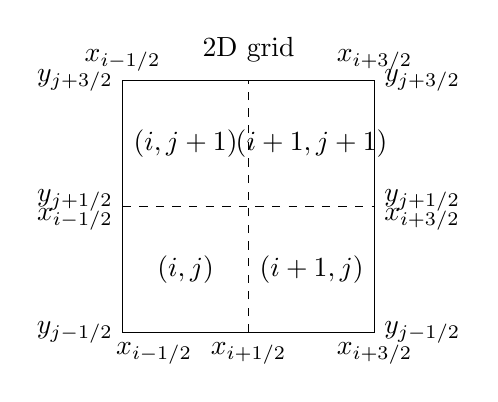
\begin{tikzpicture}[scale=0.8]
       	% Titel
       	\node at (2,4.5) {2D grid};
       % nur äußeres Quadrat
        \draw (0,0) rectangle (4,4);
      
       % Beschriftungen
        \node at (1,1) {$(i,j)$};
        \node at (3,1) {$(i+1,j)$};
        \node at (1,3) {$(i,j+1)$};
        \node at (3,3) {$(i+1,j+1)$};
      
       % Schnittlinien
        \draw[dashed] (2,0) -- (2,4);
        \draw[dashed] (0,2) -- (4,2);
       
       % optionale äußere Beschriftungen
       \node[below] at (0.5,0) {$x_{i-1/2}$};
       \node[below] at (2,0) {$x_{i+1/2}$};
       \node[below] at (4,0) {$x_{i+3/2}$};
       \node[left]  at (0,0.0) {$y_{j-1/2}$};
       \node[left]  at (0,2.1) {$y_{j+1/2}$};
       \node[left] at (0,1.8) {$x_{i-1/2}$};
       \node[left]  at (0,4) {$y_{j+3/2}$};
       \node[right]  at (4,0) {$y_{j-1/2}$};
       \node[right]  at (4,4) {$y_{j+3/2}$};
       \node[right] at (4,1.8) {$x_{i+3/2}$};
       \node[right]  at (4,2.1) {$y_{j+1/2}$};
 	   \node[above] at (0,4) {$x_{i-1/2}$};
 	   \node[above] at (4,4) {$x_{i+3/2}$};
      \end{tikzpicture}
\end{comment}

\begin{comment}
\begin{frame}{Multidimensional Wave Propagation (2D and 3D)}
	\scriptsize
	General system:
	\[
	q_t + f(q)_x + g(q)_y + h(q)_z = 0.
	\]
	
	\begin{itemize}
		\item At each cell face, solve a 1D Riemann problem in the normal direction.
		\item Decompose the jump into waves $W^p$ and corresponding speeds $s^p$.
		\item Compute fluctuations:
		\[
		\mathcal{A}^\pm \Delta q, \quad 
		\mathcal{B}^\pm \Delta q, \quad 
		\mathcal{C}^\pm \Delta q.
		\]
		\item Waves also propagate transversely:
		\begin{itemize}
			\item In 2D: a wave in $x-$direction can propagates in $y$-direction, and vice versa.
			\item In 3D: each wave generates transverse waves in the other two directions.
		\end{itemize}
	\end{itemize}
\end{frame}
\end{comment}

%-------------------------------------------------------
%-------------------------------------------------------

\begin{frame}{3D Transverse and Double Transverse Propagation}
	\scriptsize
	
    In 3D: every wave generates transverse and double–transverse contributions in the other directions

\vspace{0.5em} 
Examples of Transverse Interactions
		\begin{itemize}
			\item $x \to y$ (transverse) 
			\item $x \to z$ (transverse)
			\item $x \to y \to z$ (double transverse)
			\item $y \to x \to z$, etc.
		\end{itemize}

	\begin{block}{Update Scheme}
	\[
	\begin{aligned}
		Q_{i,j,k}^{n+1} &= Q_{i,j,k}^n
		- \frac{\Delta t}{\Delta x} \Big( \mathcal{A}^+ \Delta q_{i-1/2,j,k}
		+ \mathcal{A}^- \Delta q_{i+1/2,j,k} \Big) \\
		&\quad - \frac{\Delta t}{\Delta y} \Big( \mathcal{B}^+ \Delta q_{i,j-1/2,k}
		+ \mathcal{B}^- \Delta q_{i,j+1/2,k} \Big) \\
		&\quad - \frac{\Delta t}{\Delta z} \Big( \mathcal{C}^+ \Delta q_{i,j,k-1/2}
		+ \mathcal{C}^- \Delta q_{i,j,k+1/2} \Big).
	\end{aligned}
	\]
\end{block}
\end{frame}

%-------------------------------------------------------
%-------------------------------------------------------

\begin{comment}
\begin{frame}{Wave Propagation}
	\scriptsize
	The scheme can be specified by three integers $(m_1, m_2, m_3)$, which represent the following [LeVeque et. al]:
	\begin{align*}
		m_1 &= \left\{
		\begin{array}{ll}
			1, & \parbox[t]{0.6\textwidth}{The second order correction wave is not included,\\
				thus the method is formally first order accurate.} \\
			2, & \text{The correction wave is included.}
		\end{array}
		\right. \\
		m_2 &= \left\{
		\begin{array}{lll}
			0, & \text{No transverse propagation.} \\
			1, & \text{The propagation of the increment wave.} \\
			2, & \text{Transverse propagation of both increment and correction wave.}
		\end{array}
		\right. \\
		m_3 &= \left\{
		\begin{array}{lll}
			0, & \text{No double transverse propagation.} \\
			1, & \text{Double transverse propagation of the increment wave.} \\
			2, &  \parbox[t]{0.6\textwidth}{Double transverse propagation of both increment and \\
				correction wave.}
		\end{array}
		\right.
	\end{align*}
\end{frame}
\end{comment}